\section{Data Analysis and Results}
% description of any analytically steps: parameter estimation, error estimation, model-fitting...

\subsection{Detecting Molecular Gas Features}

We compare the final sky-subtracted and wavelength calibrated spectrum of the
Earthshine to predictions and existing measurements. First, we
detect the molecular bands of O$_2$, O$_3$, and H$_2$O by comparing the
 absorption lines obtained from \cite{nuclear}.  We verify that the abundance of
those components are compatible to the
literature (see  Fig. \ref{mol}). 

\begin{figure}[htb]
\begin{center}
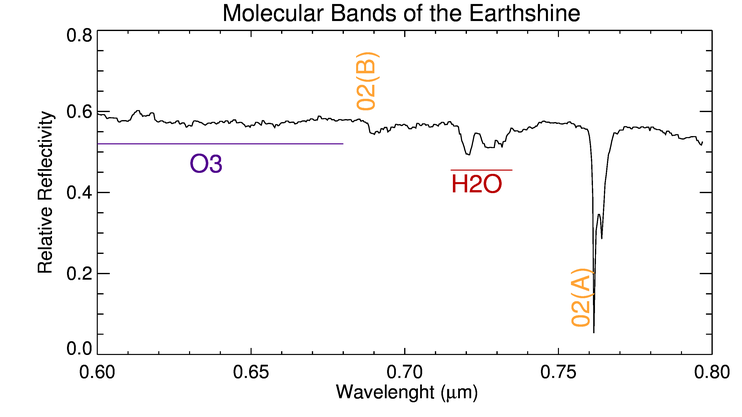
\includegraphics[scale=0.5]{plots/mo1.png}
  \caption{Atmospheric molecular bands detected in the Earthshine spectrum.}
\label{mol}
\end{center}
\end{figure}


The presence of strong
absorption lines in the near infrared when comparing to  shorter regions (blue)
of the spectra indicates that if human vision were sensitive a little further
toward the red, the natural world would be very red and exceeding bright. In the
next session we also see that the blue spectrum from the subsurface ocean water
has a very small contribution ranging for wavelengths around 500 to 600 nm.





\subsection{Detecting the Vegetation Red Edge}

The main contributors to the optical spectrum of Earthshine \cite{writeup}
\cite{USGS} are
\begin{enumerate}
 \item The {\bf neutral reflectivity from high clouds} (same as the Sun
(blackbody) with $T \sim 5700$K and independent of the wavelength).
\item The blue  spectrum of subsurface {\bf ocean water} (see Fig. \ref{veg} (right))
.
\item The {\bf transmission of Earth's  clear atmosphere}.
\item The {\bf Rayleigh scattering} (proportional to $1/\lambda^4$).
\item The {\bf vegetation} reflection spectrum from land chlorophyll
plants (see  Fig. \ref{veg} (left)).
\end{enumerate}



\begin{figure}[htb]
\begin{center}
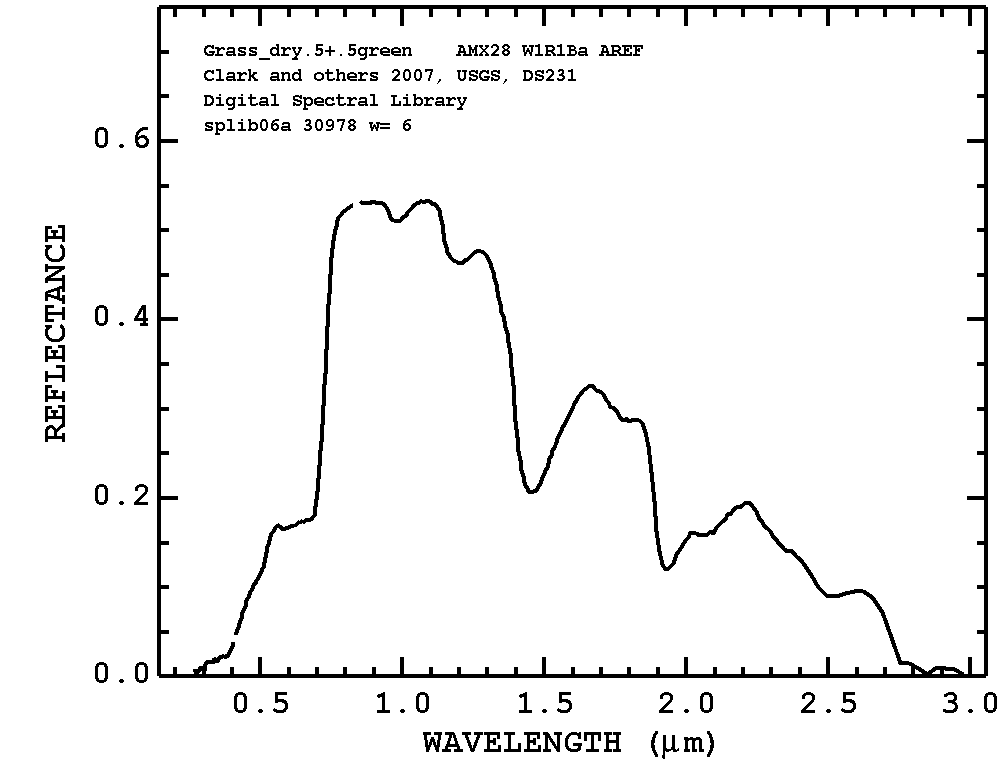
\includegraphics[scale=0.22]{figs/green.png}
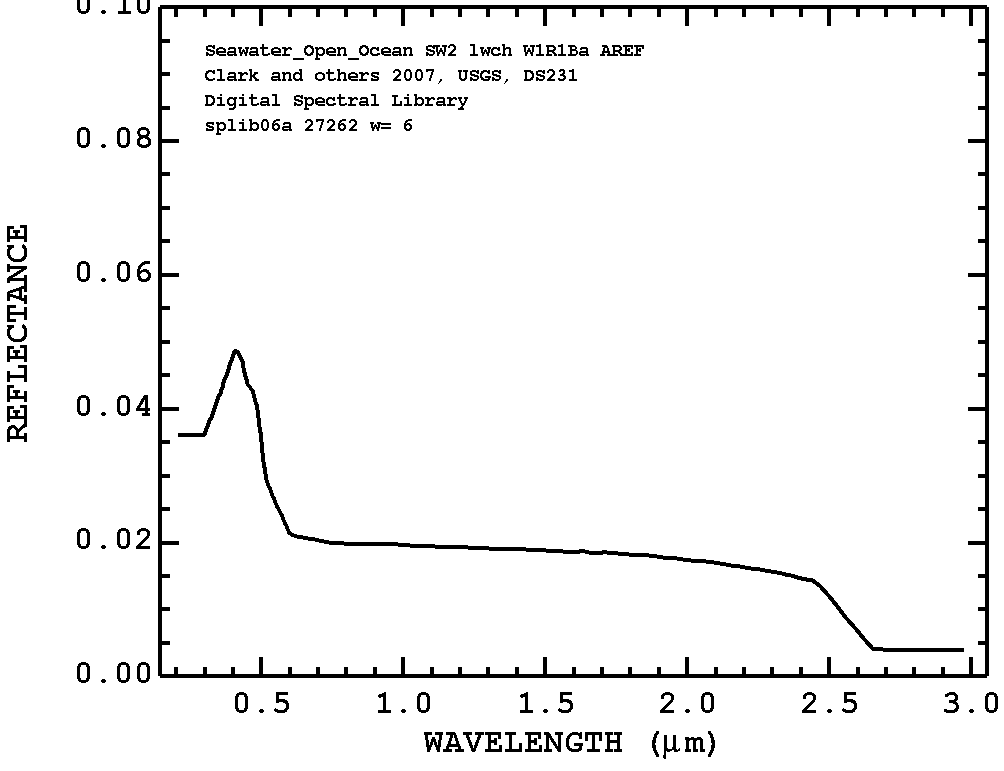
\includegraphics[scale=0.22]{figs/sea.png}
\caption{Some of the models we fitted our spectra: (left) Vegetation reflection
and (right) Ocean Surface.}
\label{veg}
\end{center}
\end{figure}

 We fit together each of the previous five models to our spectra of the
Eartshine, inferring the partial contributions to
the combined spectrum (see Fig. \ref{models}), \ie our model has 5 parameters. We calculate the best values for these parameters
to minimize $\chi^2_{point}$ on each point then integrate to an acceptable
final value of  $\chi^2=7.8$ (see fitting code in ROOT in the appendix). We
assume the data are normally distributed with a variance equal to the mean and
the data points are independent from each other, so we can use the level of
significance of $\alpha >0.1$ for the fit. For five parameters, the $\chi^2_5$
should be less than 9, so we see that our fit is indeed significant: $\chi^2$ is
not too large for a good fit and it is large enough to reject the {\it null
hypothesis} \cite{writeup}.

\begin{figure}[htb]
\begin{center}
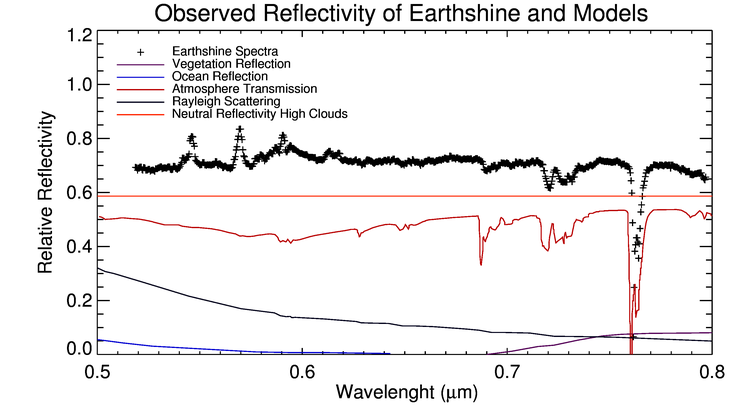
\includegraphics[scale=0.6]{plots/fit.png}
\caption{The main models to the optical spectrum of Earthshine which we fit
to our data. They are scaled in the plot for a better display.}
\label{models}
\end{center}
\end{figure}


The most important components in the fitting are the Rayleigh scattering
(high cloud continuous) in the beginning of the spectra and the clear atmosphere
(molecular spectrum) in the whole range.

We calculate the vegetation edge from equation
\ref{vge}. With mean reflectances in the [600, 670 nm] and [740, 800 nm]
windows in the spectrum, we obtain
$VGE =4 \pm 5\%$, which was small but compatible with
the literature \cite{USGS}.
The errors were estimating by looking at the standard deviation during
a ``flat'' part of the spectra and dividing by the mean in that region. 







